\documentclass{article}
\usepackage[utf8]{inputenc}
\usepackage[T1]{fontenc}
\usepackage[final]{pdfpages}
\usepackage[french]{babel}
\usepackage{colortbl}
\usepackage[table]{xcolor}
\usepackage{verbatim} 
\usepackage{graphicx}
\usepackage[left = 3.5cm, right = 3.5cm, top = 4cm, bottom = 4cm]{geometry}

\usepackage{fancyhdr}

\title{PIDR \\ \large Un protocole de lotterie en Bitcoin}
\author{Guillaume Stunault, Lucas Vignali}
\date{February 2018}

\begin{document}

\maketitle

\section{Introduction}

Pour notre projet de PIDR nous avions comme sujet : \textbf{Vérification des « smart contracts » sur la blockchain}. Ce sujet nous a été proposé par M. Jannik DREIER, membre du LORIA et de l'équipe PESTO, accompagné de M. Steve Kremer. Suite à l'essort des applications liées à la blockchain et principalement celle du Bitcoin, des règles de sécuritées comme les "Smart Contracts" doivent être mises en oeuvre pour la sureté de ces protocloles. Ces "Smart Contracts" permettent de définir et d'exécuter des contrats de façon automatique et sans besoin d'une tierce partie de confiance. Ainsi cela permet qu'aucun participant ayant signé le contrat ne se retrouve sans paiement car l'exécutions des contrats est automatique. Le but de ce PIDR a donc été de modéliser un système de smart contract. Pour cela nous avons utilisé un logiciel créé par l'équipe PESTO du LORIA : \textbf{Tamarin}. Sur ce logiciel nous avons modélisé un protocol de lotterie.


\subsection{La Blockchain}
La blockchain est une technologie de stockage et de transmission d’informations, transparente, sécurisée, et fonctionnant sans organe central de contrôle.

Par extension, une blockchain constitue une base de données qui contient l’historique de tous les échanges effectués entre ses utilisateurs depuis sa création. Ces échanges sont enregistrés sous forme de blocs, qui mis bout à bout forment une chaîne, d'où le terme blockchain. Cette base de données est sécurisée et distribuée : elle est partagée par ses différents utilisateurs, sans intermédiaire, ce qui permet à chacun de vérifier la validité de la chaîne. \cite{bcfr} \\

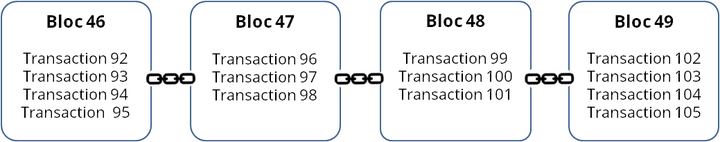
\includegraphics{blck-schema.png}

L’intérêt de la blockchain réside dans l’aspect décentralisé de la base de données qui est stockée sur les différents serveurs des utilisateurs et fonctionne sans intermédiaire ce qui limite les frais d’infrastructure. Cette base de données que beaucoup comparent à un grand livre comptable – public et partagé – contient un historique infalsifiable des transactions qui est mis à jour en temps réel par les utilisateurs. Les utilisateurs valident chaque transaction et vérifient la cohérence de celle-ci grâce au registre. \\

\textbf{Pourquoi infalsifiable ? } \\
Distribuée, et non centralisée, la base de données est aussi doublement sécurisée. D'abord par un système de cryptographie dite "asymétrique". Cela signifie simplement qu'il faut deux clés différentes (une privée, une publique) pour soumettre une transaction dans la blockchain. Ensuite, Chaque bloc est validé par les noeuds du réseau appelés les “mineurs”. Les "mineurs" chargés de vérifier la validité des transactions bloc par bloc sont des particuliers, rémunérés pour mettre à disposition la puissance de calcul de leurs processeurs en résolvant des fonctions de hachage cryptographique. Dans la blockchain du Bitcoin, cette technique s'appelle le "Proof-of-Work" (preuve de travail). \cite{7x7} \\
Ainsi pour manipuler la blockchain, il faudrait pouvoir falsifier plus de la motité des noeuds du sytème, ce qui correspond à hacker des milliers d'utilisateurs au même moment. Techniquement, il s’agit d’une prouesse impossible. \\
\begin{center}
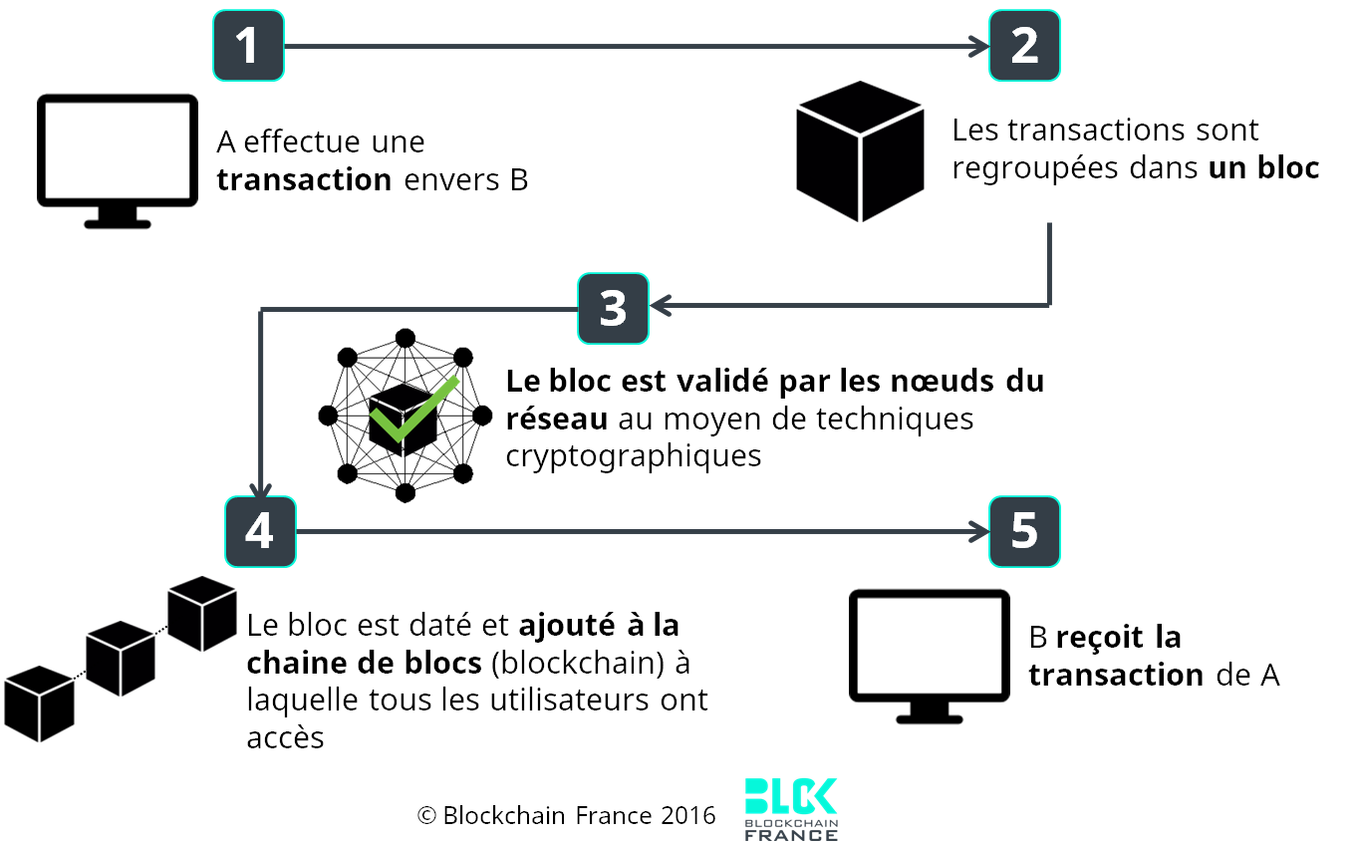
\includegraphics[scale=0.4]{blck-fonctionnement.png}
\end{center}
\\
\textbf{Le potentiel de la blockchain} \cite{bcfr}\\

Bien que souvent associé au Bitcoin et autres cryptomonnaies, le caractère décentralisé de la blockchain, couplé avec sa sécurité et sa transparence, promet des applications bien plus larges : 
\begin{itemize}
    \item Les applications pour le transfert d’actifs (utilisation monétaire, mais pas uniquement : titres, votes, actions, obligations…)
    \item Les applications de la blockchain en tant que registre : elle assure ainsi une meilleure traçabilité des produits et des actifs.
    \item Les smart contracts : il s’agit de programmes autonomes qui exécutent automatiquement les conditions et termes d’un contrat, sans nécessiter d’intervention humaine une fois démarrés. 
\end{itemize} 

\newpage

\subsection{Le Bitcoin}

Le Bitcoin est une monnaie virtuelle mais aussi un sytème de paiement pair à pair. C'est la prmière monnaie électronique décentralisé. Ce type de monnaie possède différent avantages : 
\begin{itemize}
    \item Echange de particulier à particulier ce qui implique des frais inférieurs aux banques
    \item Utilisable dans tous les pays
    \item Les comptes ne peuvent pas être gelés
    \item Pas de conditions
\end{itemize}

Les bitcoins peuvent être générés par toute personne possédant un ordinateur et faisant tourner un logiciel appelé "mineur de bitcoin". Cette création de bitcoin requiert de de travailler sur chaque bloc de transaction. Ceci est ajusté par le réseau pour que la création des bitcoin soit prédictible et limitée. Enfin les bitcoin sont stockés dans des portes monnaies électroniques. Chaque transaction est vérifiée puis stockée sur le réseau.

\subsection{Notions cryptographiques}

\section{Le protocole de lotterie}
Nous allons analysé un protocole de smart contract qui implémente une lotterie Bitcoin. \cite{955}
Ce protocole garantit :
\begin{itemize}
\item chaque joueur honnête aura (en moyenne) un gain non négatif, même dans le
présence d'adversaires qui jouent contre 
\item Si tous les joueurs sont honnetes, le protocole simule une lotterie ordinaire : 1 joueur remporte les mises des autres joueurs 
\end{itemize}
Le protocole utilise un arbre de tournoi : chaque manche le gagnant remporte la mise de l'adversaire \\
\\ \\

Initialisation : \\
\begin{itemize}
\item chaque joueur génère N paires de clés, O(N\up{2}) signatures (N signatures pour N paires de clé * N transactions Win, Timeout... pour chaque joueur) et log(N) secrets qu'il hash ensuite pour tous les matchs qu'il va jouer.
\item on vérifie que les hashs ne sont pas réutilisés
\item ensuite il pose la mise en signant une transaction Init
\item si un joueur ne pose pas la mise, les autres récupèrent leur mise
\item Init est ajouté à la blockchain
\item La transaction doit s'effectuer dans un temps donné, assez long pour qu'il permette la transaction. Ce temps est calculé pour permettre la géneration des clés 
\item Init est ensuite séparée en N mises de départ : Win(p,p) ajoutées à la blockchain \\
\end{itemize}
\\
Execution :  \\
\begin{itemize}
\item C'est la phase de match, soient $\pi_{k}$ le match actuel, $p_{1}$ et $p_{2}$ les joueurs qui s'affrontent
\item Au départ, on ajoute à la blockchain, les transactions Win( $\pi_{k-1}$, $p_{1}$) et Win( $\pi_{k-1}$, $p_{2}$) si ça n'a pas déjà été fait
\item $p_{1}$ commence, on ajoute Turn1($\pi_{k}$, $p_{1}$, $p_{2}$) à la blockchain :  $p_{1}$ doit donc révéler son secret à temps en l'ajoutant, comme in-scipt dans Turn2($\pi_{k}$, $p_{1}$, $p_{2}$)
\item Ainsi, $p_{2}$ peut vérifier que le hash de $p_{1}$ correspond au hash envoyé au départ
\item $p_{2}$ connait son propre secret et exécute la fonction aléatoire w = winner($\pi_{k}$, $p_{1}$, $p_{2}$, $Sk_{1}$, $Sk_{2}$)
\item $p_{2}$ ajoute finalement à la blockchain la transaction Win(w, $\pi_{k}$) avec pour in-script son secret $Sk_{2}$.
\item Chaque joueur doit chacun son tour réveler sa clé dans un temps imparti sinon il perd. \\
\end{itemize}
\\
Mise : \\
 A tous les tours, chaque joueur mise 1 bitcoin. Pour éviter la fraude et qu'un joueur quitte la partie en plein milieu avec l'argent qu'il a récolté, chaque joueur pose au début une somme de bitcoins égale au nombre de parties possibles par un joueur. Ainsi à chaque partie gagné un bitcoin est retiré de cette somme, et si le joueur quitte la partie en plein milieu cette est reversé à chaque joueur afronté précedement ce qui fait que le joueur en question ne gagne pas d'argent. Dans le cas ou il perd une manche cette mise lui est rendu.

\section{Protocole réalisé}
Nous avons simplifié le protocole au maximum pour tester ses divers propriétés de sécurité. \\
Nous prenons désormais uniquement 2 joueurs A et B, et une seule manche de match. \\
La mise vaut pour le moment : 1 bitcoin \\
De plus, pour modéliser la blockchain, nous considérons les traces de Tamarin. En effet, la blockchain rend les transactions enregistrées consultables à chaque moment tout comme les traces de Tamarin.


\begin{itemize}
    \item A et B génèrent chacun une clé publique et une clé secrète
    \item A partir de cette clé secrète, le protocole assigne un porte-monnaie avec 3 bitcoins à chaque joueur
    \item Chacun des 2 joueurs génère ensuite un secret pour le match, et envoie son hash signé sur le réseau.
    \item La blockchain retire 1 Bitcoin du porte-monnaie de A et B pour créer une mise
    \item La blockchain crée un contrat où A et B posent leurs mises. Lorsque les 2 mises sont posées, le match peut commencer.
    \item La blockchain crée un contrat où A doit révéler son secret. Elle vérifie que le hash du secret envoyé correspond au hash envoyé avant le match
    \item Idem pour B
    \item Lorsque la blockchain possède les 2 hashs, elle peut déterminer aléatoirement un gagnant entre A et B.
    \item La blockchain ajoute les 2 Bitcoins au porte-monnaie du gagnant.
\end{itemize}

Normalement, la blockchain est censé déterminer un gagnant avec une fonction sur la parité des secrets (processus qui est défini aléatoire et non truquable). Pour modéliser cela sur Tamarin, nous avons crée 2 règles identiques de victoire : une avec A, une avec B. Et Tamarin choisit aléatoirement une de ces 2 règles.

\section{Propriétés à prouver}
\begin{itemize}
    \item Il existe une exécution normale du protocole
    \item A la fin, le porte-monnaie de l'un contient 4 bitcoins, et celui du perdant 2 bitcoins
    
\end{itemize}




\begin{comment}
 N = 2^(L) joueurs
 2^(L)-1 = N-1 1v1 joués
 pi = numéro du matchh
\end{comment}





\newpage
\begin{tabular}{|m{3cm}|m{7cm}}
\hline
\rowcolor{grey!40} \textbf{Date} & \textbf{Travail effectué}  \\ 
\hline 
\rowcolor{grey!10}  07/02/2018 & Découverte du sujet \\
\hline
\rowcolor{grey!10}  14/02/2018 & Installation de Tamarin \newline Choix du protocole : Lotterie \\
\hline
\rowcolor{grey!10}  15/03/2018 & Compréhension du sujet \newline Rédaction du rapport \newline Découverte Tamarin \\
\hline
\rowcolor{grey!10}  04/04/2018 & Première version compilable du protocole \\
\end{tabular}


\newpage
\bibliographystyle{plain-fr}
\bibliography{bibliography.bib}
\end{document}


